\documentclass[aspectratio=169,10pt]{beamer}

\usetheme{Madrid}
\usecolortheme{seahorse}

\usepackage{amsmath}
\usepackage{amssymb}
\usepackage{amsfonts}
\usepackage{graphicx}
\usepackage{listings}
\usepackage{xcolor}
\usepackage{hyperref}
\usepackage{subcaption}

\graphicspath{{figures/}}

% Define theorem-like environments
\usebeamertemplate{theorems}
\newtheorem{proposition}{Proposition}
\newtheorem{example}{Example}
\newtheorem{definition}{Definition}

% Code style
\lstset{
    basicstyle=\ttfamily\scriptsize,
    numbers=left,
    numberstyle=\tiny\color{gray},
    stepnumber=1,
    frame=single,
    backgroundcolor=\color{white},
    keywordstyle=\color{blue},
    commentstyle=\color{green!50!black}\itshape,
    stringstyle=\color{red},
    breaklines=true,
}

% Footer
\setbeamertemplate{footline}[frame number]

% Title page
\title{Chapter 21: Finer Monotone Properties}
\subtitle{Convex Analysis and Monotone Operator Theory (2nd ed., 2017)}
\author{Bauschke \& Combettes}
\date{Lecture Notes}

\begin{document}

% ============================================================================
% Title Slide
% ============================================================================
\begin{frame}[plain]
    \titlepage
\end{frame}

% ============================================================================
% Outline
% ============================================================================
\begin{frame}[allowframebreaks]{Outline}
    \tableofcontents
\end{frame}

% ============================================================================
% Introduction
% ============================================================================
\section{Introduction: Maximally Monotone Operators}

\begin{frame}{Core Concepts}
    \begin{itemize}
        \item \textbf{Monotone Operator}: $A: H \to 2^H$ is monotone if
        \[
            \langle x - y, u - v \rangle \geq 0 \quad \text{for all } (x,u), (y,v) \in \text{gra } A
        \]

        \item \textbf{Maximally Monotone}: A monotone operator $A$ such that no proper
        monotone extension exists

        \item \textbf{Graph}: $\text{gra } A = \{(x, u) \mid u \in A(x)\}$

        \item \textbf{Domain}: $\text{dom } A = \{x \in H \mid A(x) \neq \emptyset\}$

        \item \textbf{Range}: $\text{ran } A = \{u \in H \mid \exists x: u \in A(x)\}$
    \end{itemize}

    \begin{center}
        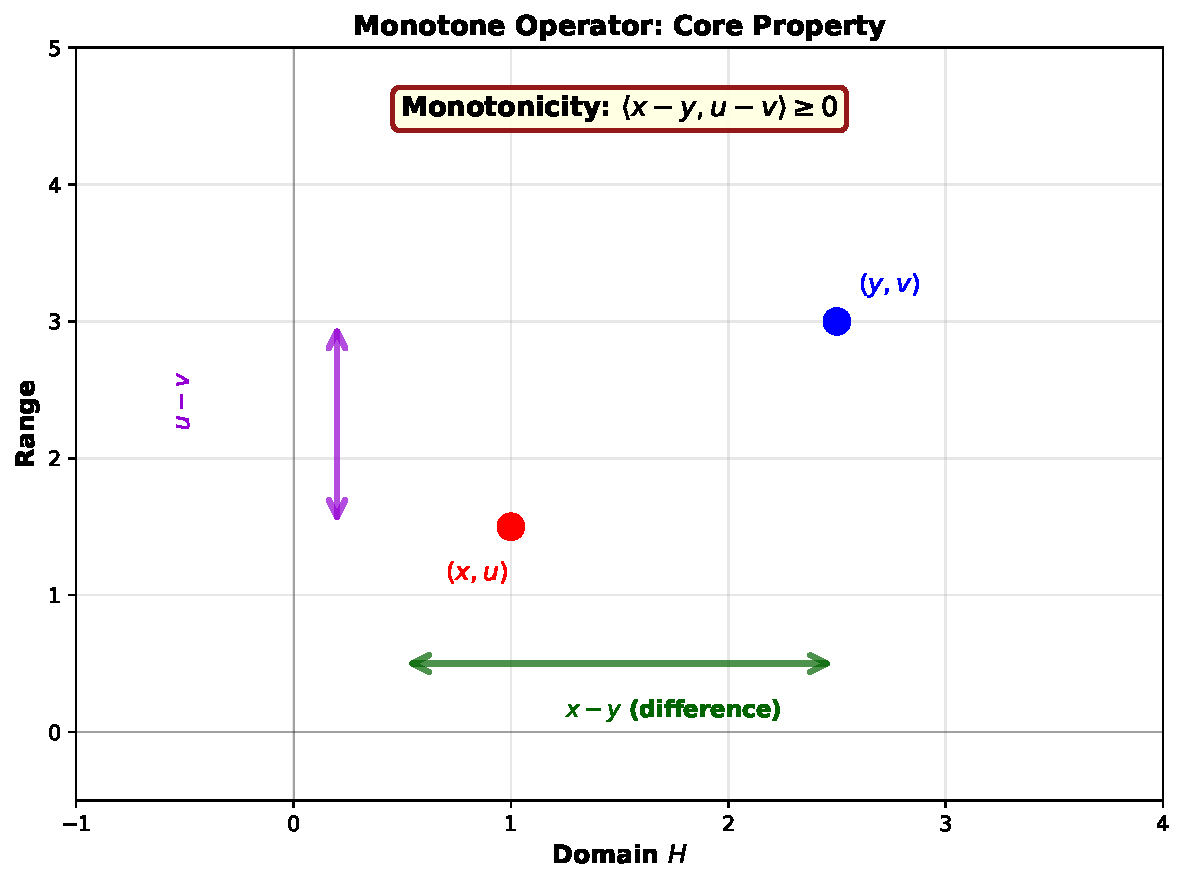
\includegraphics[width=0.5\textwidth]{fig_monotone_property}
    \end{center}
\end{frame}

% ============================================================================
% Section 21.1: Minty's Theorem
% ============================================================================
\section{Section 21.1: Minty's Theorem}

\begin{frame}{Theorem 21.1: Maximal Monotonicity Characterization}
    \begin{theorem}[Theorem 21.1]
        Let $A: H \to 2^H$ be monotone. Then $A$ is maximally monotone if and only if
        \[
            0 \in \text{ran}(A + \text{Id}).
        \]
    \end{theorem}

    \begin{proof}[Proof Sketch]
        \begin{itemize}
            \item[\(\Rightarrow\)] If $A$ is maximally monotone, then $\text{ran}(A + \text{Id}) = H$
            \item[\(\Leftarrow\)] If $0 \in \text{ran}(A + \text{Id})$ for all monotone extensions,
                 maximality follows from the equivalence to Proposition 20.56
        \end{itemize}
    \end{proof}

    \vspace{1em}
    \textbf{Consequence}: For maximally monotone $A$: $\boxed{\text{ran}(A + \text{Id}) = H}$
\end{frame}

\begin{frame}{Minty's Theorem: Intuition and Example}
    \begin{definition}[Minty's Theorem]
        If $A: H \to 2^H$ is maximally monotone, then the operator $T = \text{Id} + A$ is
        surjective: $\text{ran}(T) = H$.
    \end{definition}

    \vspace{0.5em}
    \textbf{Example 21.3}: Let $\mathcal{K}$ be a real Hilbert space, $L \in \mathcal{B}(H, \mathcal{K})$.
    Set $T = \text{Id} + L^\ast L$ and $R = \text{Id} + LL^\ast$.

    \textbf{Result}: $T: H \to H$ and $R: \mathcal{K} \to \mathcal{K}$ are bijective with continuous inverses
    (from Theorem 21.1 and properties of $L^\ast L$).

    \begin{center}
        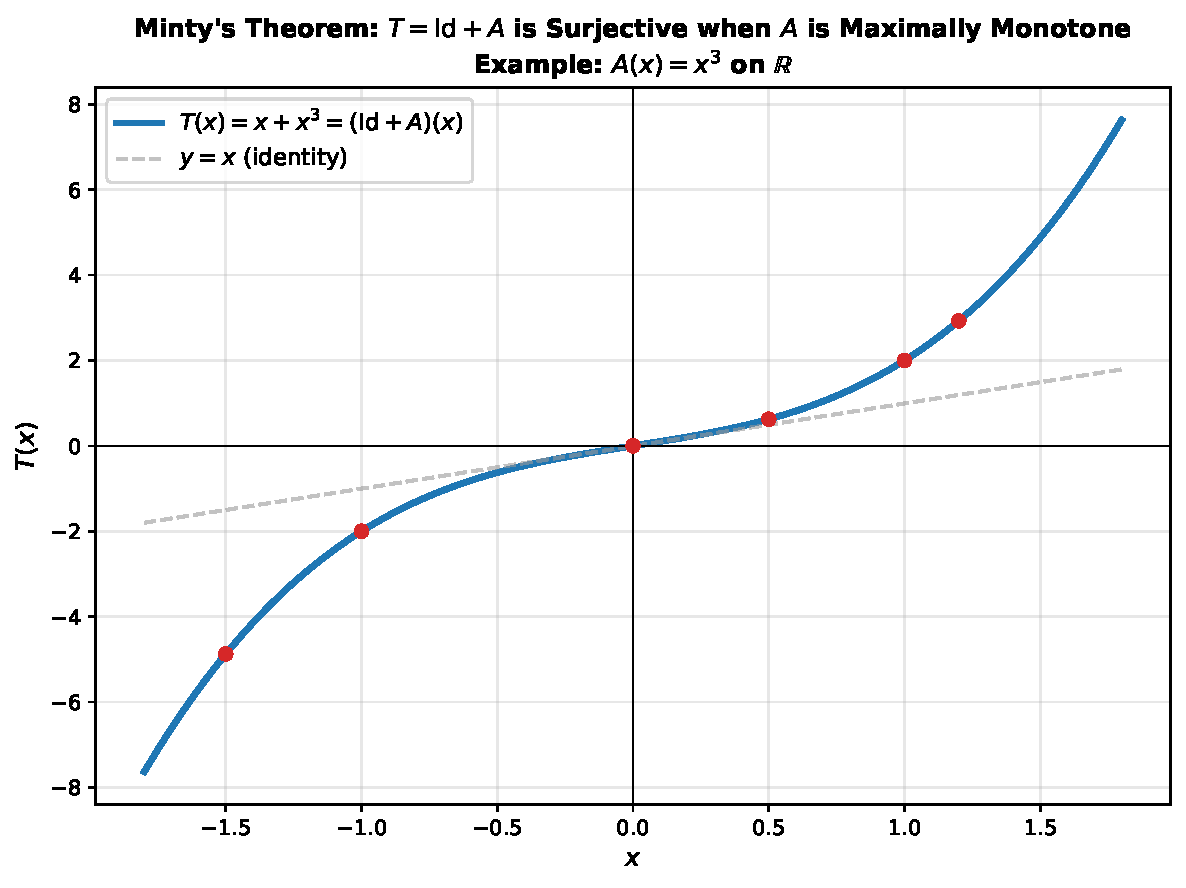
\includegraphics[width=0.6\textwidth]{fig_minty}
    \end{center}
\end{frame}

\begin{frame}{Applications of Minty's Theorem}
    \begin{theorem}[Theorem 21.2]
        Let $f \in \Gamma_0(H)$. Then $\partial f$ is maximally monotone.
    \end{theorem}

    \textbf{Proof}: Combine Example 20.3, Proposition 16.45, and Theorem 21.1.

    \vspace{1em}
    \begin{proposition}[Proposition 21.4]
        Let $H = L^2([0,T]; H)$ and let $A$ be the time-derivative operator:
        \[
            A(x) = \begin{cases} \{x'\} & \text{if } x \in W^{1,2}([0,T]; H) \text{ and } x(0) = x_0 \\
                   \emptyset & \text{otherwise} \end{cases}
        \]
        Then $A$ is maximally monotone.
    \end{proposition}

    \vspace{1em}
    \begin{proposition}[Proposition 21.5]
        Let $C$ be a nonempty compact convex subset of $H$. Then $-\phi_C$ is maximally monotone,
        where $\phi_C$ is the farthest-point operator.
    \end{proposition}
\end{frame}

% ============================================================================
% Section 21.2: Debrunner-Flor Theorem
% ============================================================================
\section{Section 21.2: The Debrunner-Flor Theorem}

\begin{frame}{Theorem 21.8: The Debrunner-Flor Separation Theorem}
    \begin{theorem}[Debrunner-Flor Theorem]
        Let $A: H \to 2^H$ be a monotone operator such that $\text{gra } A \neq \emptyset$. Then
        \[
            \left(\forall w \in H\right) \quad \left(\exists x \in \overline{\text{conv dom } A}\right) \quad
            0 \leq \inf_{(y,v) \in \text{gra } A} \langle y - x \mid v - (w - x) \rangle.
        \]
    \end{theorem}

    \textbf{Key Consequence}:
    \begin{theorem}[Theorem 21.9: Maximal Monotone Extension]
        Let $A: H \to 2^H$ be monotone. Then there exists a maximally monotone extension $\bar{A}$
        of $A$ such that $\text{dom } \bar{A} \subseteq \overline{\text{conv dom } A}$.
    \end{theorem}
\end{frame}

\begin{frame}{Debrunner-Flor: Proof and Intuition}
    \begin{itemize}
        \item The Debrunner-Flor theorem provides a \textbf{separation property} for monotone sets

        \item For every point $w \in H$, there exists a point $x$ in the closure of the
              convex hull of the domain such that the infimum of inner products is non-negative

        \item This is used to show existence of maximally monotone extensions
    \end{itemize}

    \begin{center}
        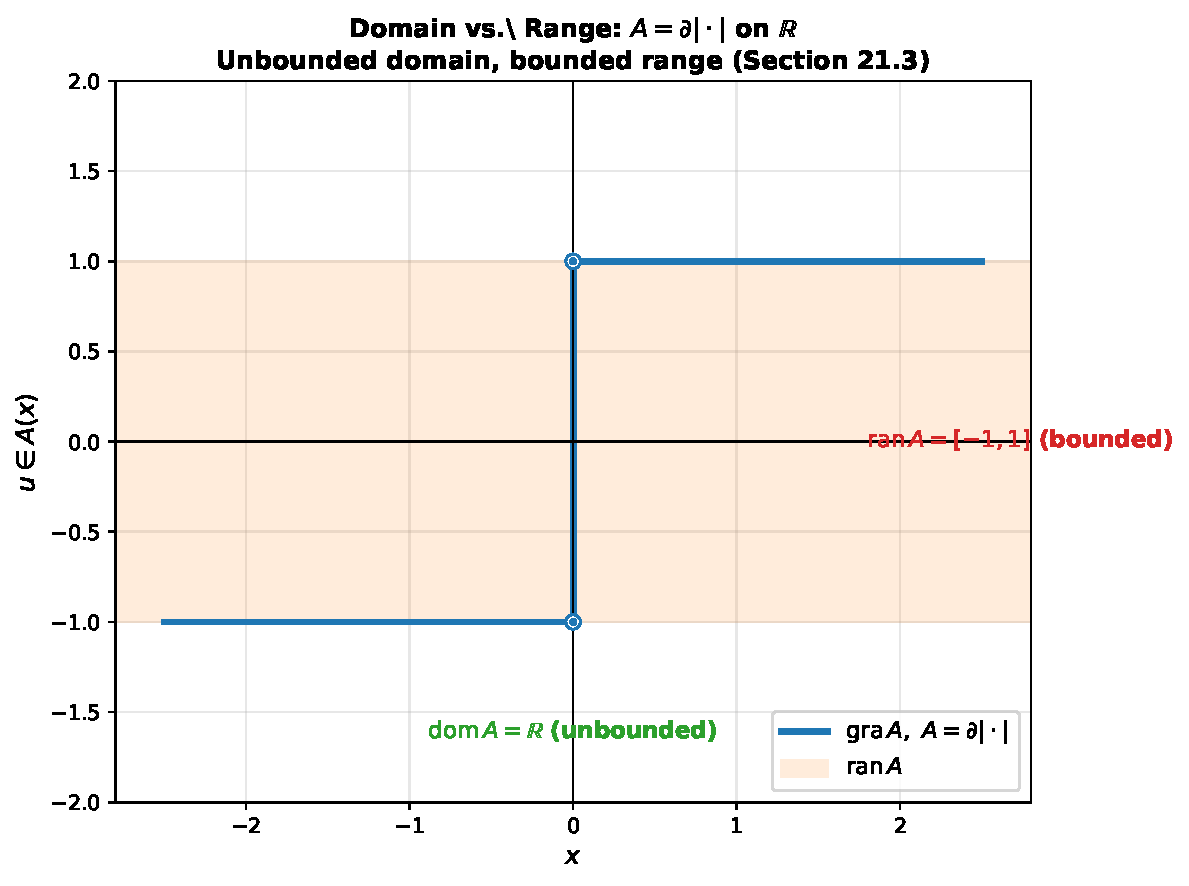
\includegraphics[width=0.7\textwidth]{fig_domain_range}
    \end{center}
\end{frame}

% ============================================================================
% Section 21.3: Domain and Range
% ============================================================================
\section{Section 21.3: Domain and Range}

\begin{frame}{Definition 21.10: Local Boundedness}
    \begin{definition}[Local Boundedness]
        Let $A: H \to 2^H$ and let $x \in H$. Then $A$ is \textbf{locally bounded at } $x$
        if there exists $\delta \in \mathbb{R}_{++}$ such that $A(B(x; \delta))$ is bounded.
    \end{definition}

    \vspace{1em}
    \begin{proposition}[Proposition 21.11]
        Let $A: H \to 2^H$ be monotone, set $Q_1: H \times H \to H: (x,u) \mapsto x$,
        and suppose that $z \in \text{int } Q_1(\text{dom } F_A)$. Then $A$ is locally bounded at $z$.
    \end{proposition}

    \vspace{1em}
    \textbf{Interpretation}: Interior points of the domain projection are points of local boundedness
\end{frame}

\begin{frame}[allowframebreaks]{Proposition 21.12: Domain Relations}
    \begin{proposition}[Proposition 21.12]
        Let $A: H \to 2^H$ be maximally monotone and set $Q_1: H \times H \to H: (x,u) \mapsto x$.
        Then
        \[
            \text{int dom } A \subset \text{int } Q_1(\text{dom } F_A) \subset \text{dom } A \subset Q_1(\text{dom } F_A) \subset \overline{\text{dom } A}.
        \]

        Consequently, $\text{int dom } A = \text{int } Q_1(\text{dom } F_A)$ and
        $\text{dom } A = Q_1(\text{dom } F_A)$.

        If $\text{int dom } A \neq \emptyset$, then $\text{int dom } A = \text{dom } A$.
    \end{proposition}

    \pagebreak

    \begin{example}[Example 21.13]
        Let $C$ be a nonempty closed convex subset of $H$ and set $Q_1: H \times H \to H: (x,u) \mapsto x$.
        Then $Q_1(\text{dom } F_{N_C}) = C$.
    \end{example}

    \begin{corollary}[Corollary 21.14: Convexity of Domain and Range]
        Let $A: H \to 2^H$ be maximally monotone, and set $Q_1$ and $Q_2$ as above. Then
        \[
            \text{dom } A = Q_1(\text{dom } F_A), \quad \text{int dom } A = \text{int } Q_1(\text{dom } F_A),
        \]
        \[
            \overline{\text{ran } A} = Q_2(\text{dom } F_A), \quad \text{int ran } A = \text{int } Q_2(\text{dom } F_A).
        \]

        Consequently, the sets $\text{dom } A$, $\text{int dom } A$, $\overline{\text{ran } A}$,
        and $\text{int ran } A$ are convex.
    \end{corollary}
\end{frame}

\begin{frame}{Bunt-Kritikos-Motzkin Result}
    \begin{corollary}[Corollary 21.16: Bunt-Kritikos-Motzkin]
        Suppose that $H$ is finite-dimensional and let $C$ be a Chebyshev subset of $H$.
        Then $C$ is closed and convex.
    \end{corollary}

    \textbf{Proof}: Uses Remark 3.11(i), Example 20.33, and Corollary 21.14 applied to
    the farthest-point operator.

    \vspace{1em}
    \textbf{Consequence}: In finite dimensions, Chebyshev sets (closest-point unique)
    must be closed and convex.
\end{frame}

% ============================================================================
% Section 21.4: Local Boundedness and Surjectivity
% ============================================================================
\section{Section 21.4: Local Boundedness and Surjectivity}

\begin{frame}{Proposition 21.17: Recession Cones}
    \begin{proposition}[Proposition 21.17]
        Let $A: H \to 2^H$ be maximally monotone and let $x \in \text{dom } A$.
        Then $\text{rec}(Ax) = N_{\overline{\text{dom } A}}^x$.
    \end{proposition}

    \vspace{1em}
    \textbf{Interpretation}: The recession cone of $A(x)$ equals the normal cone to the closure
    of the domain at $x$.

    \vspace{1em}
    \begin{theorem}[Theorem 21.18: Rockafellar-Vesely]
        Let $A: H \to 2^H$ be maximally monotone and let $x \in H$. Then $A$ is locally bounded at $x$
        if and only if $x \notin \text{bdry } \text{dom } A$.
    \end{theorem}

    \textbf{Key Fact}: Local boundedness characterizes interior points of the domain.
\end{frame}

\begin{frame}{Rockafellar-Vesely Example}
    \begin{center}
        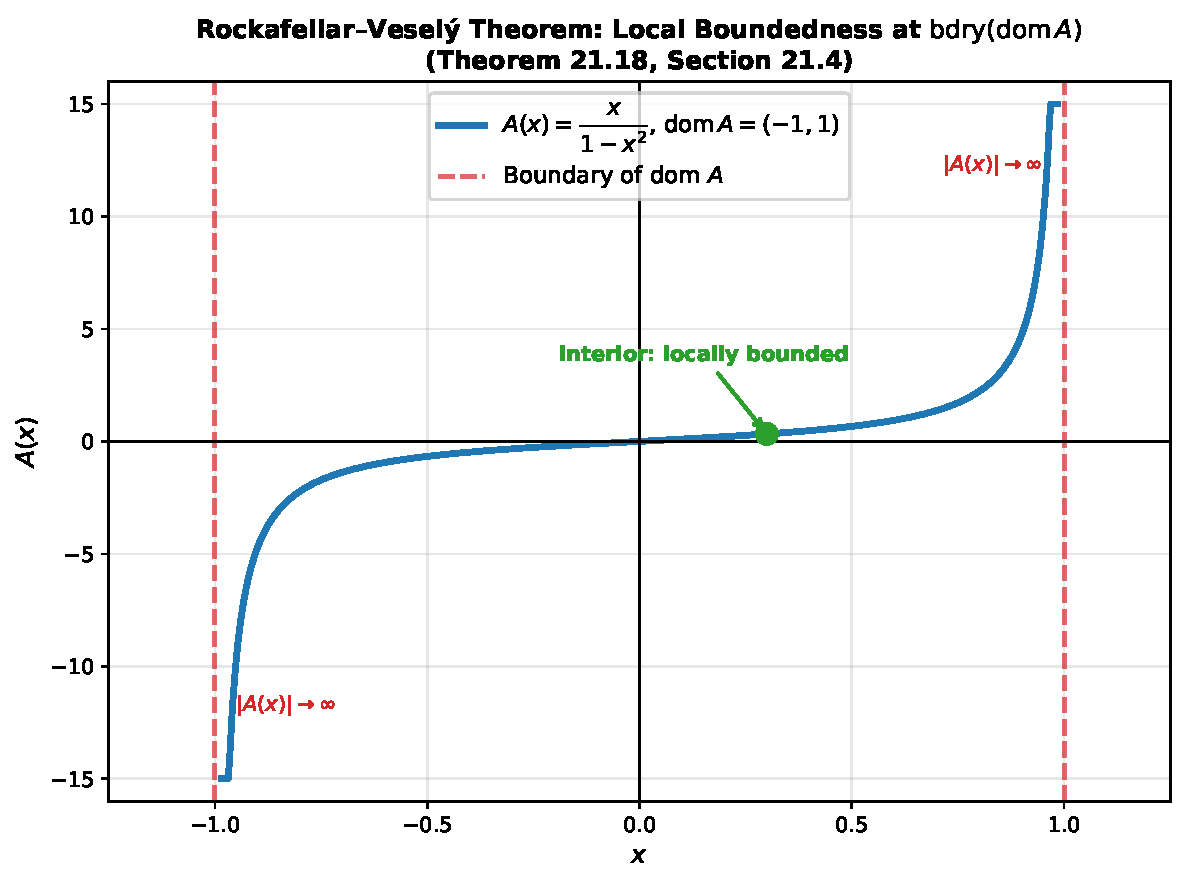
\includegraphics[width=0.8\textwidth]{fig_local_bdd}
    \end{center}

    \textbf{Example}: $A(x) = \frac{x}{1-x^2}$ on $(-1,1)$ shows that $|A(x)| \to \infty$
    as $x$ approaches the boundary $\pm 1$.
\end{frame}

\begin{frame}[allowframebreaks]{Surjectivity Corollaries}
    \begin{corollary}[Corollary 21.19]
        Let $A: H \to 2^H$ be monotone, and suppose that $C$ is a compact subset of $\text{int dom } A$.
        Then $A(C)$ is bounded.
    \end{corollary}

    \begin{corollary}[Corollary 21.20]
        Let $A: H \to 2^H$ be maximally monotone. Then $A$ is locally bounded everywhere on $H$
        if and only if $\text{dom } A = H$.
    \end{corollary}

    \pagebreak

    \begin{corollary}[Corollary 21.21]
        Let $A: H \to 2^H$ be maximally monotone and at most single-valued. Then $A$ is
        strong-to-weak continuous everywhere on $\text{int dom } A$.
    \end{corollary}

    \vspace{1em}
    \textbf{Key Results on Surjectivity}:

    \begin{corollary}[Corollary 21.23]
        Let $A: H \to 2^H$ be maximally monotone. Then $A$ is surjective if and only if
        $A^{-1}$ is locally bounded everywhere on $H$.
    \end{corollary}

    \begin{corollary}[Corollary 21.24]
        Let $A: H \to 2^H$ be a maximally monotone operator such that
        \[
            \lim_{\|x\| \to +\infty} \inf \|Ax\| = +\infty.
        \]
        Then $A$ is surjective.
    \end{corollary}

    \begin{corollary}[Corollary 21.25]
        Let $A: H \to 2^H$ be maximally monotone with bounded domain. Then $A$ is surjective.
    \end{corollary}
\end{frame}

\begin{frame}{Application to Convex Functions}
    \begin{corollary}[Corollary 21.26]
        Let $f \in \Gamma_0(H)$ and let $C$ be a compact subset of $\text{int dom } f$.
        Then $\partial f(C)$ is bounded.
    \end{corollary}

    \textbf{Consequence}: Subdifferentials of convex functions are locally bounded on
    the interior of their domains.
\end{frame}

% ============================================================================
% Section 21.5: Kenderov's Theorem
% ============================================================================
\section{Section 21.5: Kenderov's Theorem and Fréchet Differentiability}

\begin{frame}[allowframebreaks]{Theorem 21.27: Kenderov's Theorem}
    \begin{theorem}[Kenderov's Theorem - Theorem 21.27]
        Let $A: H \to 2^H$ be a maximally monotone operator such that
        $\text{int dom } A \neq \emptyset$. Then there exists a subset $C$ of $\text{dom } A$
        that is a dense $G_\delta$ subset of $\text{int dom } A$ such that, for every point $x \in C$:

        \begin{enumerate}
            \item $Ax$ is a singleton
            \item Every selection of $A$ is continuous at $x$
        \end{enumerate}
    \end{theorem}

    \vspace{1em}
    \textbf{Key Implications}:
    \begin{itemize}
        \item On a dense subset, the multi-valued operator becomes single-valued
        \item Every selection (any choice of element from $A(x)$) is continuous at those points
        \item This is a generic property (holds on a dense $G_\delta$ set)
    \end{itemize}

    \pagebreak

    \textbf{Proof Strategy}:
    \begin{itemize}
        \item Use a sequence $(\varepsilon_n)_{n \in \mathbb{N}}$ converging to $0$
        \item Define sets $C_n$ by requiring $y \in C_n$ iff diameter of $A(V) < \varepsilon_n$
              for some open neighborhood $V$ of $y$
        \item Show each $C_n$ is open in $\text{int dom } A$
        \item Show $C = \bigcap_{n \in \mathbb{N}} C_n$ is the required dense $G_\delta$ set
        \item On $C$, the operator is single-valued and every selection is continuous
    \end{itemize}
\end{frame}

\begin{frame}{Application to Convex Functions: Fréchet Differentiability}
    \begin{corollary}[Corollary 21.28]
        Let $f \in \Gamma_0(H)$ be such that $\text{int dom } f \neq \emptyset$. Then there exists
        a subset $C$ of $\text{int dom } f$ such that $C$ is a dense $G_\delta$ subset of
        $\text{dom } f$, and such that $f$ is Fréchet differentiable on $C$.
    \end{corollary}

    \vspace{1em}
    \textbf{Interpretation}:
    \begin{itemize}
        \item Convex functions with nonempty interior domain are generically Fréchet differentiable
        \item Differentiability holds on a dense $G_\delta$ subset (measure-theoretically "most" points)
        \item This is the sharpest result possible: there exist convex functions with no
              point of Gâteaux differentiability (see Example 21.6)
    \end{itemize}

    \vspace{1em}
    \textbf{Generic Property}: The set of points where Fréchet differentiability holds
    is not just nonempty—it is dense and of full "category" in the Baire sense.
\end{frame}

\begin{frame}{Example 21.6: A Convex Function with Limited Differentiability}
    \begin{example}[Example 21.6]
        Let $\mathbb{P} = \mathbb{N} \setminus \{0\}$, $H = \ell^2(\mathbb{P})$,
        let $(e_n)_{n \in \mathbb{P}}$ be the canonical orthonormal basis, and set
        \[
            f: H \to [-\infty, +\infty]: x \mapsto \max\left\{1 + \langle x, e_1 \rangle,
                \sup_{2 \leq n \leq N} \langle x, \sqrt{n}e_n \rangle\right\}.
        \]

        Then $f \in \Gamma_0(H)$ and $\partial f$ is maximally monotone. However,
        $\text{gra } \partial f$ is not closed in $H^{\text{strong}} \times H^{\text{weak}}$.
    \end{example}

    \vspace{1em}
    \textbf{Note}: This example shows that even though $\partial f$ is maximally monotone,
    its graph may not be closed when considering different topologies.
\end{frame}

% ============================================================================
% Numerical Example
% ============================================================================
\section{Numerical Examples}

\begin{frame}[fragile]{Python Implementation: Monotone Operator Analysis}
    \begin{lstlisting}[language=Python]
import numpy as np
from scipy.optimize import fminbound

# Example: A(x) = subdifferential of f(x) = ||x||^2/2
class SubdifferentialNorm:
    def f(self, x):
        """Convex function: f(x) = 0.5 * ||x||^2"""
        return 0.5 * np.sum(x**2)

    def A(self, x):
        """Subdifferential: partial f(x) = x (single-valued)"""
        return x

    def verify_monotonicity(self, x1, x2):
        """Verify: <x1-x2, A(x1)-A(x2)> >= 0"""
        u1, u2 = self.A(x1), self.A(x2)
        return np.dot(x1 - x2, u1 - u2) >= -1e-10

# Test monotonicity
A = SubdifferentialNorm()
x1 = np.array([1.5, 2.0])
x2 = np.array([0.5, 1.0])
is_monotone = A.verify_monotonicity(x1, x2)
print(f"Monotone: {is_monotone}")  # True
print(f"Inner product: {np.dot(x1-x2, A(x1)-A(x2)):.4f}")
    \end{lstlisting}
\end{frame}

\begin{frame}{Visualization of Example Operator}
    \begin{center}
        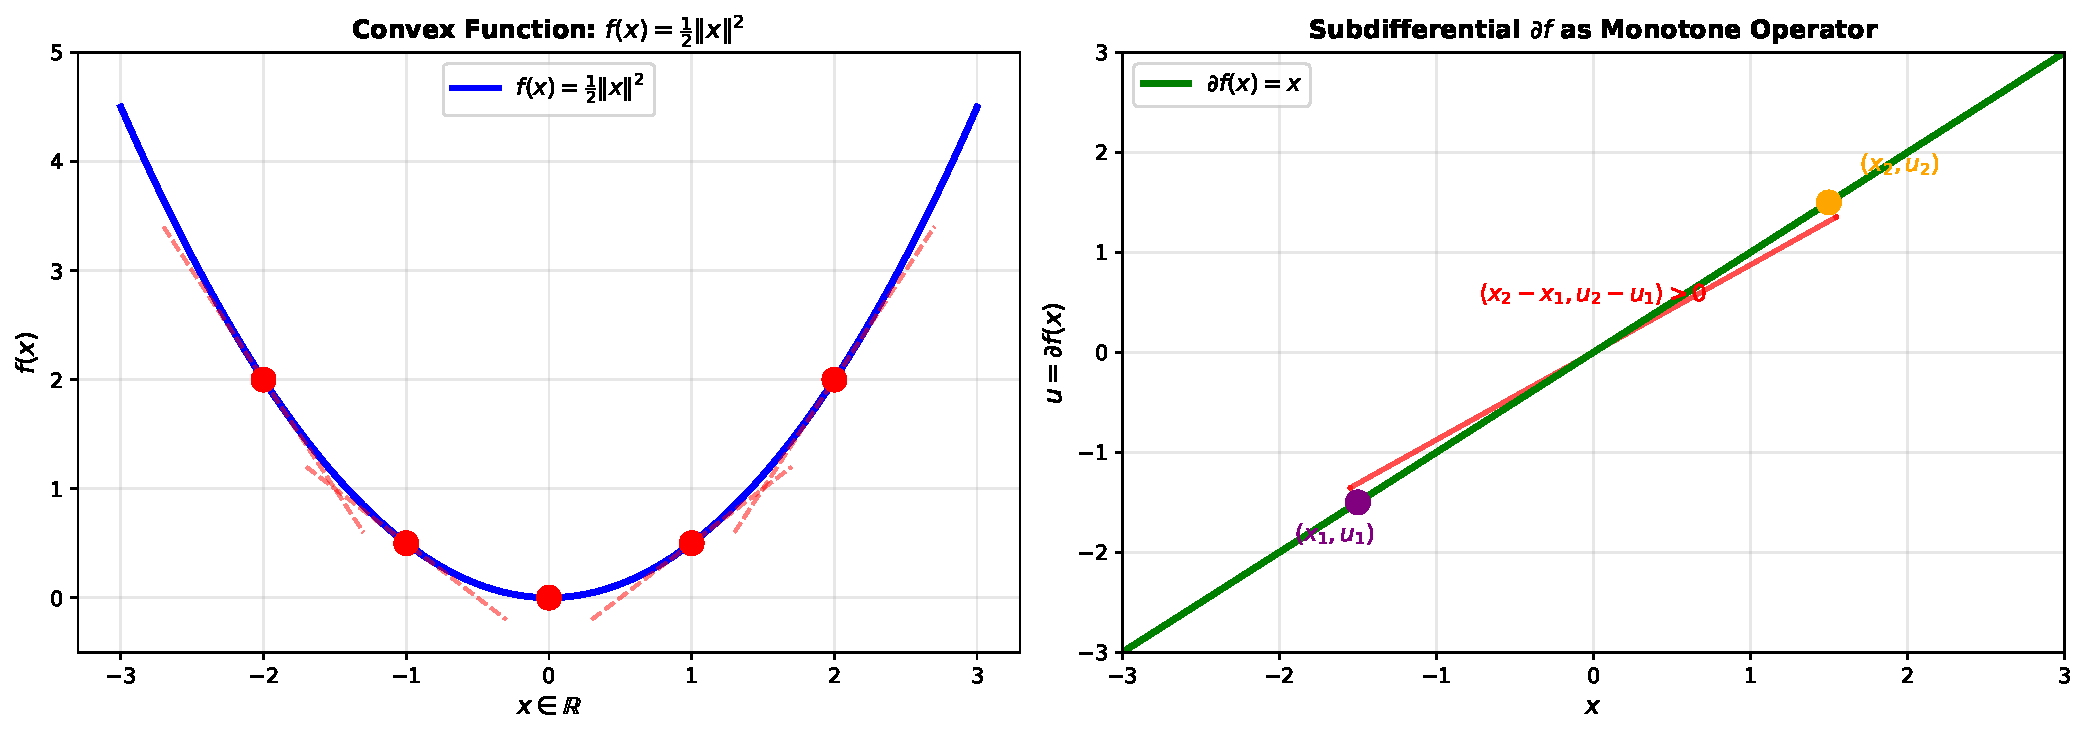
\includegraphics[width=0.95\textwidth]{fig_example_operator}
    \end{center}

    The subdifferential $\partial f$ of the convex function $f(x) = \frac{1}{2}\|x\|^2$
    is the linear monotone operator $x \mapsto x$.
\end{frame}

% ============================================================================
% Summary
% ============================================================================
\section{Summary and Key Takeaways}

\begin{frame}{Summary: Five Main Themes}
    \begin{center}
        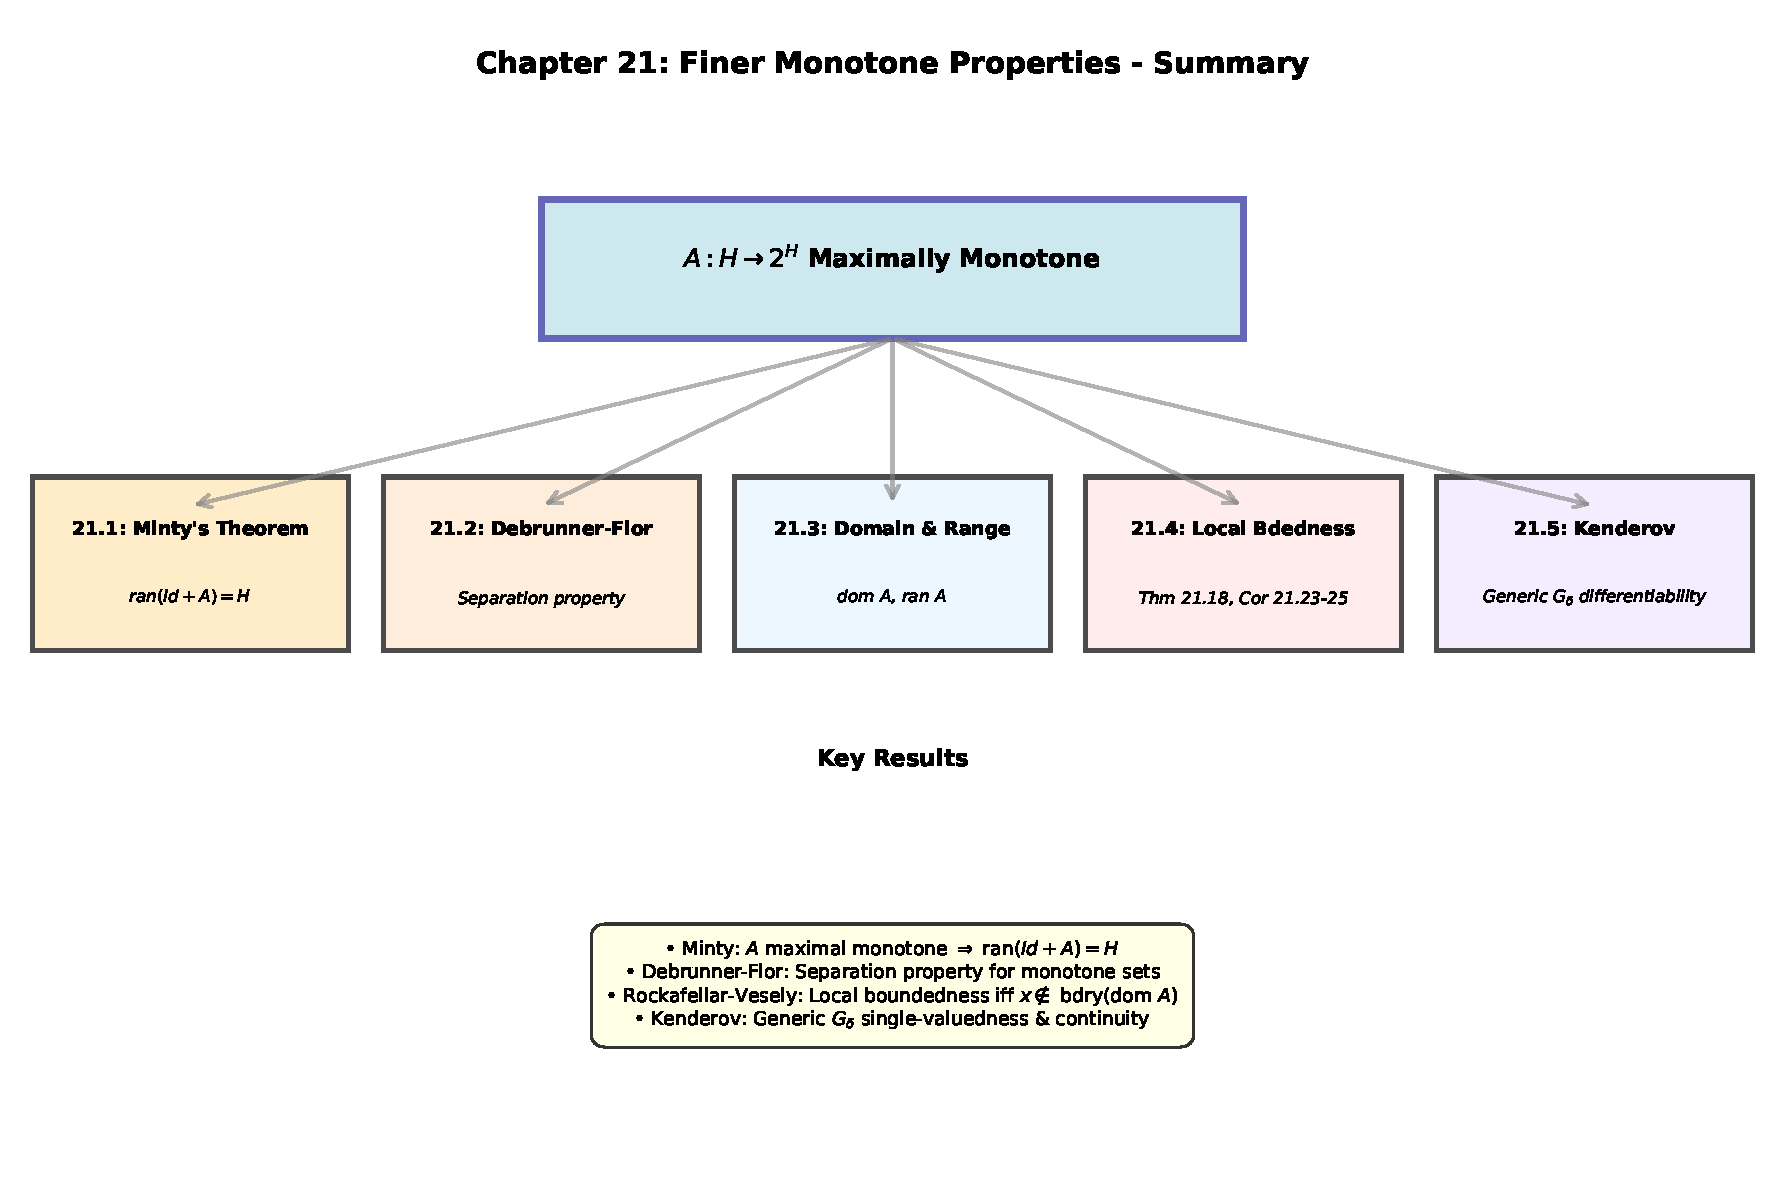
\includegraphics[width=\textwidth]{fig_summary}
    \end{center}
\end{frame}

\begin{frame}[allowframebreaks]{Key Theorems and Results}
    \begin{enumerate}
        \item \textbf{Theorem 21.1}: Maximal monotonicity is equivalent to $0 \in \text{ran}(A + \text{Id})$

        \item \textbf{Minty's Theorem}: If $A$ is maximally monotone, then
              $\text{ran}(\text{Id} + A) = H$

        \item \textbf{Debrunner-Flor Theorem}: Provides a separation property for monotone sets
              and characterizes maximal monotone extensions

        \item \textbf{Domain-Range Relations}: For maximally monotone $A$ with
              $\text{int dom } A \neq \emptyset$:
              - $\text{dom } A = \overline{\text{dom } A}$ and $\text{int dom } A = \text{dom } A$
              - Both $\text{dom } A$ and $\text{ran } A$ are convex

        \pagebreak

        \item \textbf{Local Boundedness}: (Rockafellar-Vesely, Theorem 21.18)
              - $A$ is locally bounded at $x \iff x \notin \text{bdry } \text{dom } A$

        \item \textbf{Surjectivity Conditions}:
              - $A$ surjective $\iff$ $A^{-1}$ locally bounded everywhere
              - If $\lim_{\|x\| \to \infty} \inf \|Ax\| = +\infty$, then $A$ surjective
              - If $\text{dom } A$ bounded, then $A$ surjective

        \item \textbf{Kenderov's Theorem}: For maximally monotone $A$ with
              $\text{int dom } A \neq \emptyset$:
              - There exists a dense $G_\delta$ subset $C$ of $\text{dom } A$
              - On $C$: $Ax$ is singleton and every selection is continuous

        \item \textbf{Fréchet Differentiability}: Convex functions with nonempty interior domain
              are Fréchet differentiable on a dense $G_\delta$ subset
    \end{enumerate}
\end{frame}

\begin{frame}{Connections to Other Chapters}
    \begin{itemize}
        \item \textbf{Chapter 16}: Single-valued subdifferentials and continuous selections

        \item \textbf{Chapter 20}: Properties of convex functions (from which these results are applied)

        \item \textbf{Chapter 21}: Finer properties of monotone operators beyond basic characterizations

        \item \textbf{Chapter 22}: Stronger notions of monotonicity
              (para-, strict, uniform, strong monotonicity)

        \item \textbf{Applications}: Optimization algorithms, evolution equations, variational inequalities
    \end{itemize}
\end{frame}

% ============================================================================
% Exercises and Further Study
% ============================================================================
\section{Exercises and Further Study}

\begin{frame}{Key Exercises from Chapter 21}
    \begin{itemize}
        \item \textbf{Exercise 21.1}: Show that $A$ is maximally monotone iff $\text{gra } A + \text{gra}(-\text{Id}) = H \times H$

        \item \textbf{Exercise 21.2}: Matrix monotonicity (for symmetric matrices)

        \item \textbf{Exercise 21.3}: Distance to graph using Gâteaux differentiability

        \item \textbf{Exercise 21.5}: Equivalence of maximal monotonicity with:
              (i) Strong-to-weak continuity
              (ii) Hemicontinuity

        \item \textbf{Exercise 21.6}: Subdifferentials of Gâteaux differentiable functions

        \item \textbf{Exercise 21.12}: Finite-dimensional result on bounded subsets

        \item \textbf{Exercise 21.17}: Fréchet differentiability instances (at what sets of points)
    \end{itemize}
\end{frame}

\begin{frame}{Further Reading}
    \begin{itemize}
        \item \textbf{Minty (1962)}: Original work on maximally monotone operators and their properties

        \item \textbf{Rockafellar (1970)}: Monotone operators and convex analysis

        \item \textbf{Bauschke \& Combettes (2017)}: Comprehensive modern treatment with
              Hilbert space setting

        \item \textbf{Zarantonello (1971)}: Solving Functional Equations by Contraction Mappings

        \item \textbf{Brezis (1973)}: Opérateurs Maximaux Monotones et Semi-groupes de Contractions
    \end{itemize}
\end{frame}

% ============================================================================
% Closing
% ============================================================================
\begin{frame}[plain]
    \begin{center}
        \Large
        \textbf{Chapter 21: Finer Monotone Properties} \\[1em]
        \normalsize
        Maximally monotone operators form a powerful framework for\\
        convex analysis and the study of operator equations.\\[2em]

        The results presented here—Minty, Debrunner-Flor, Rockafellar-Vesely,
        and Kenderov—are\\
        fundamental tools for modern optimization and variational analysis.
    \end{center}
\end{frame}

\end{document}
